% model_lda.tex
%
% Copyright (C) 2010,2011 Laura Dietz
% Copyright (C) 2012 Jaakko Luttinen
%
% The MIT License
%
% See LICENSE file for more details.

% Latent Diriclet allocation model
\documentclass{standalone}
\usepackage{tikz}
\usetikzlibrary{bayesnet}

\begin{document}
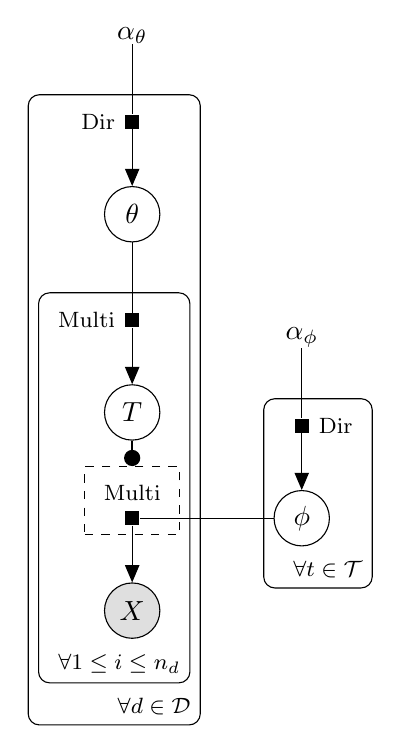
\begin{tikzpicture}[x=1.7cm,y=1.8cm]

    % Nodes
  
    \node[obs]                   (X)      {$X$} ; %
    \node[latent, above=of X]    (T)      {$T$} ; %
    \node[latent, above=of T]    (theta)  {$\theta$}; %
    \node[const, above=of theta] (atheta) {$\alpha_\theta$};
  
  
    % Factors
    \factor[above=of X]     {X-f}     {Multi} {} {} ; %
    \factor[above=of T]     {T-f}     {left:Multi} {} {} ; %
    \factor[above=of theta] {theta-f} {left:Dir} {} {} ; %
  
    % More nodes
    \node[latent, right=of X-f] (phi)  {$\phi$}; %
    \node[const, above=of phi]  (aphi) {$\alpha_\phi$}; %
  
    \factor[above=of phi] {phi-f} {right:Dir} {} {} ; %
  
    \factoredge {theta}  {T-f}     {T} ; %
    \factoredge {atheta} {theta-f} {theta} ; %
    \factoredge {phi}    {X-f}     {X} ; %
    \factoredge {aphi}   {phi-f}   {phi} ; %
  
    \gate {X-gate} {(X-f)(X-f-caption)} {T}
  
    \plate {plate1} { %
      (X)(X-gate) %
      (T)(T-f)(T-f-caption) %
    } {$\forall 1 \leq i \leq n_d$}; %
    \plate {} { %
      (plate1) %
      (theta)(theta-f)(theta-f-caption) %
    } {$\forall d \in \mathcal{D}$} ; %
    \plate {} { %
      (phi)(phi-f)(phi-f-caption) %
    } {$\forall t \in \mathcal{T}$} ; %
  
\end{tikzpicture}
\end{document}
